\begin{center}
    \textbf{6. АЛГОРИТМ РЕШЕНИЯ ЗАДАЧИ И ЧИСЛЕННЫЕ ПРИМЕРЫ}
\end{center}

Представим алгоритм решения задачи управления.
Заметим, что в соответствии с~\eqref{OC2} градиент функционала качества равен
\[
    J'_\lambda (u) = \lambda u - p_2.
\]
Здесь $u\in U$ -- управление в граничном условии~\eqref{bc1}, $p_2$ -- соответствующая компонента
сопряженного состояния из системы~\eqref{OC1}--\eqref{OC2}.

Предлагаемый алгоритм решения задачи (CP) выглядит следующим образом:
\begin{algorithm}[H]
    \caption{Алгоритм градиентного спуска}
    \begin{algorithmic}[1]
        \State Выбираем значение градиентного шага $\varepsilon$,
        \State Выбираем количество итераций $N$,
        \State Выбираем произвольное $u_0 \in U$,
        \For{$k \gets 0,1,2,\dots,N$}
            :
            \State Для полученного $u_k$ расчитываем состояние $y_k = \{\theta_k, \varphi_k\}$ из~\eqref{eq1}.
            \State Расчитываем значение функционала качества $J(\theta_k, u_k)$ из~\eqref{cost}.
            \State Расчитываем состояние $p_k=\{p_{1k},p_{2k}\}$ из уравнений~\eqref{OC1},
            где $ \hat{\theta} := \theta_k, \hat{u}=u_k$.
            \State Пересчитываем управление $u_{k+1} = u_k - \varepsilon (\lambda u_k - p_2)$
        \EndFor
    \end{algorithmic}
\end{algorithm}
Значение параметра $\varepsilon$ выбирается эмпирически таким образом, чтобы значение
$\varepsilon (\lambda u_k - p_2)$ являлась существенной поправкой для $u_{k+1}$.
Количество итераций $N$ выбирается достаточным для выполнения условия
$J(\theta_k, u_k) - J(\theta_{k+1}, u_{k+1}) < \delta$, где $\delta>0$ задает точность расчетов.

Примеры, рассмотренные ниже, иллюстрируют эффективность предложенного алгоритма даже при
малых значениях параметра регуляризации $\lambda < 10^{-12}.$

\textbf{Для численного решения прямой задачи с заданным управлением и сопряженной системы
использовался солвер FEniCS~\cite{fenics, dolfin}.}
%    Исходные коды расчётов для настоящей статьи представлены по адресу \url{https://github.com/mesenev/articles_src}


Приведем примеры расчетов для куба с ребром $l=1~\text{см}$,
$\Omega = {(x, y, z), 0 \leq x,y,z \leq l}$.
Будем также далее считать, что $a = 0.006[\text{см}^2/\text{c}]$,
$b=0.025[\text{см}/\text{с}]$, $\beta = 0.00005[\text{см}/\text{с}]$,
$\kappa=1[\text{см}^{-1}]$, $\kappa_s = 0$, $A = 0$, $\gamma = 0.3$.
Указанные параметры соответствуют стеклу~\cite{Grenkin5}. \textbf{Параметр регуляризации $\lambda=10^{-12}.$}


\textbf{Пример 1.}
Пусть граничные данные $r$ и $u$ в~\eqref{bc1} имеют вид:
\begin{gather*}
    r = 0.8 cos(x) + 0.1,\quad
    u = \hat u = y.
\end{gather*}
Далее рассчитываем состояние $\theta$ и $\varphi$ как решение задачи~\eqref{eq1}--\eqref{bc1} и в качестве
$\theta_b$ выбираем граничные значение функции $\theta$ на $\Gamma$.
Применяя предложенный алгоритм с начальным приближением $u_0 = 0.1$ находим приближенное решение задачи CP\@.
Квадрат разницы тестового и найденного решения,
а также динамика функционала качества представлена на рисунке~\ref{img_test_1}.

\begin{figure}[H]
    \centering
    \subfloat[ $(\hat u - u_{100})^2$]
    {
        \label{fig1:exp1}
        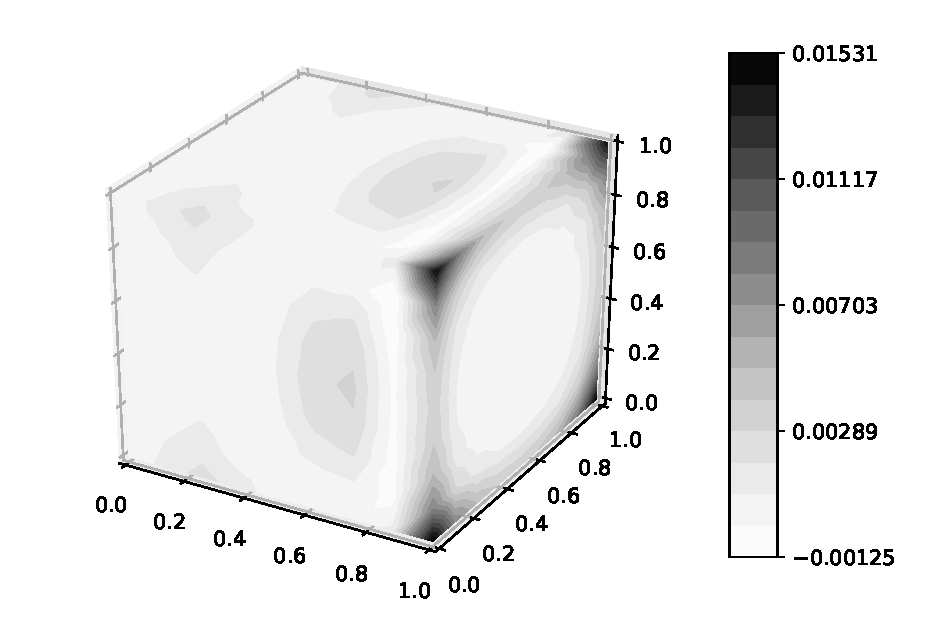
\includegraphics[width=.49\linewidth]{img/exp1/diff_end_control}
    }
    \subfloat[Изменение функционала в зависимости от числа итераций]
    {
        \label{fig1:exp2}
        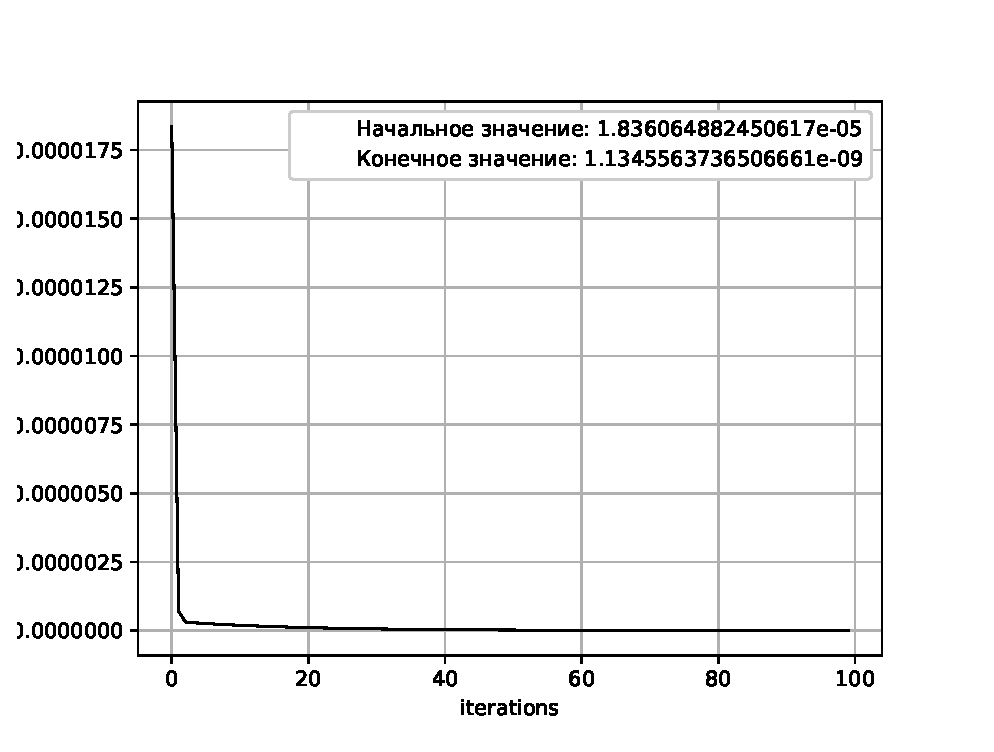
\includegraphics[width=.49\linewidth]{img/exp1/quality}
    }
    \caption{Пример 1.}
    \label{img_test_1}
\end{figure}

\textbf{Пример 2.}
Для второго эксперимента вместо тестовой функции управления $u$
определим функции $\theta_b$, $q_b$ из~\eqref{bc2} следующим образом
\[
    \theta_b = 0.1z + 0.3, \;
    q_b =
    \begin{cases}
        0.11, & \text{если } z = 1,\\
        0, & \text{если } 0 < z < 1,\\
        -0.15, & \text{если } z = 0.
    \end{cases}
\]

В данном примере оптимальное управление $u$ в качестве тестового не задается.
На рисунке~\ref{img_test_2} представлен результат работы алгоритма

\begin{figure}[H]
    \centering
    \subfloat[Найденное оптимальное управление]
    {
        \label{fig2:exp1}
        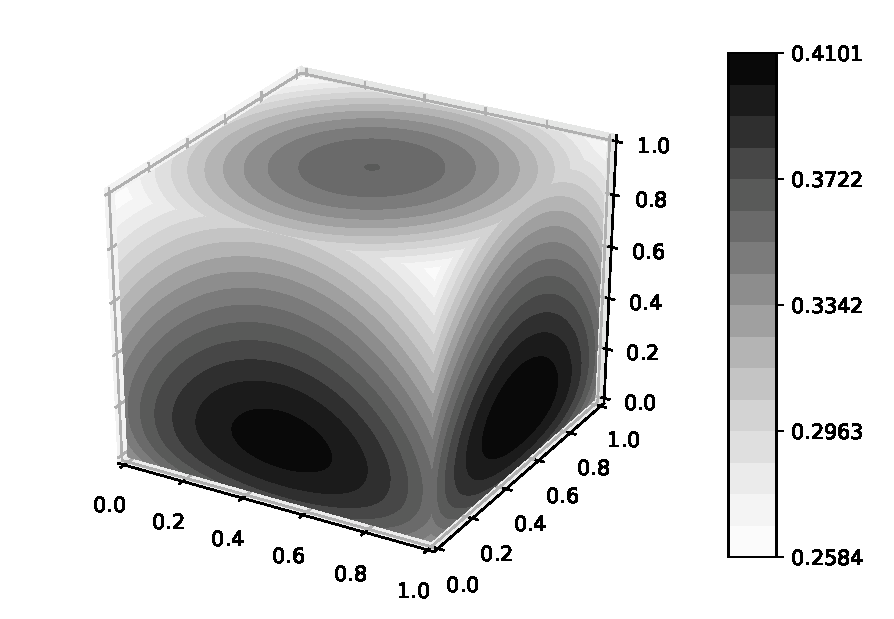
\includegraphics[width=.49\linewidth]{img/exp2/end_control}
    }
    \subfloat[Изменение функционала в зависимости от числа итераций]
    {
        \label{fig2:exp2}
        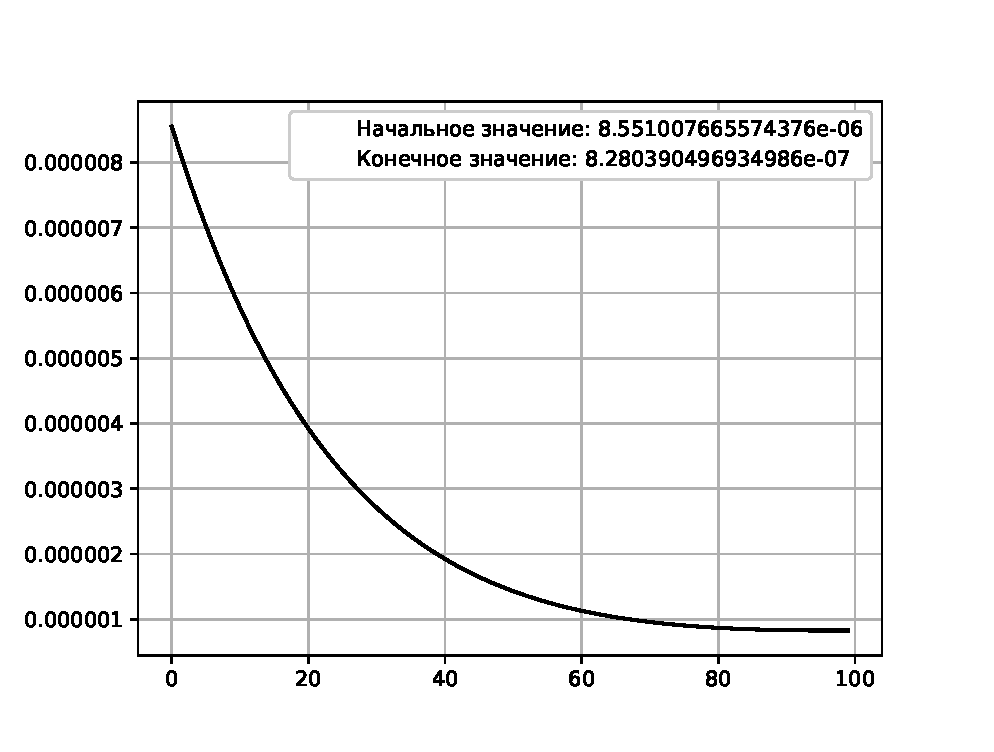
\includegraphics[width=.49\linewidth]{img/exp2/quality}
    }
    \caption{Пример 2.1}
    \label{img_test_2}
\end{figure}

Компоненты состояния, соотвествующие найденному управлению представлены на рисунке~\ref{img_end_state}.
\begin{figure}[H]
    \centering
    \subfloat[Температурa $\theta$]
        {
        \label{fig3:exp2}
        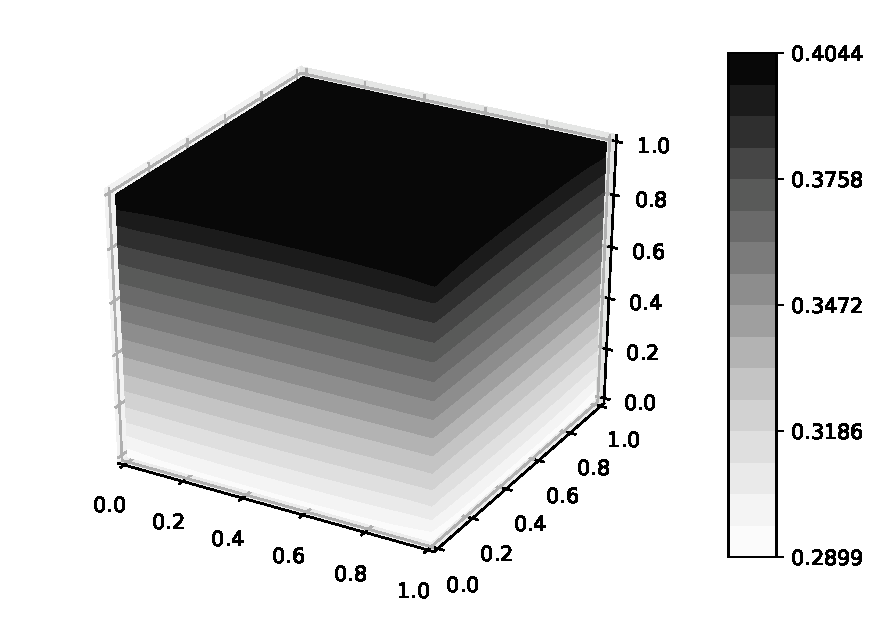
\includegraphics[width=.49\linewidth]{img/exp2/end_theta}
    }
    \subfloat[Излучение $\varphi$]
        {
        \label{fig4:exp2}
        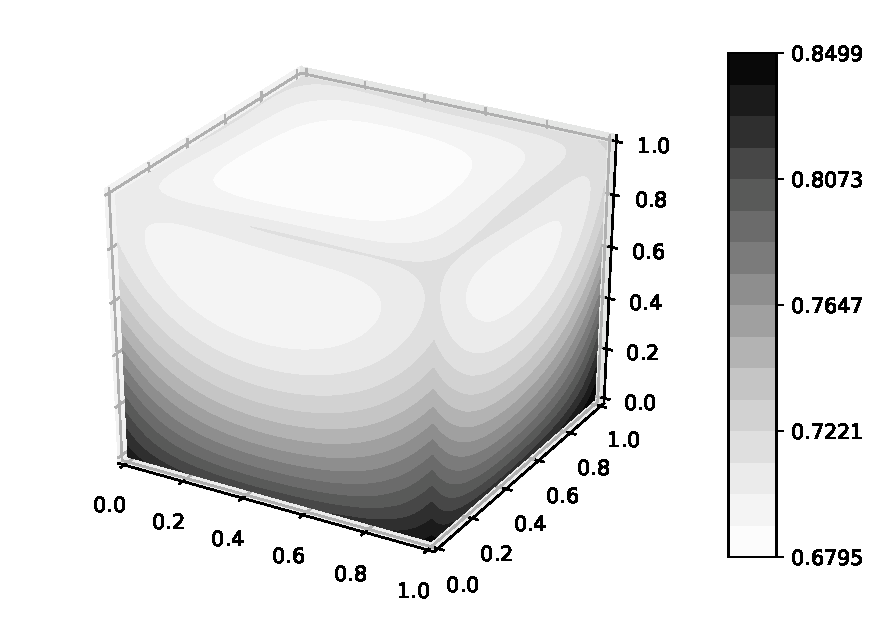
\includegraphics[width=.49\linewidth]{img/exp2/end_phi}
    }
    \caption{Пример 2.2}
    \label{img_end_state}
\end{figure}
